\documentclass[article,type=bsc,colorback,accentcolor=tud9c]{tudthesis}
\usepackage[english]{babel}
\usepackage{amsmath}
\usepackage{amssymb}
\usepackage{hyperref}
\usepackage{booktabs}
\usepackage{tabularx}
\usepackage{subfig}
\usepackage{pgf}
\usepackage{enumitem}
\setenumerate{itemsep=0.4pt,topsep=14pt,parsep=10pt,partopsep=14pt}

\thesistitle{Text classification using concept maps}{}
\author{David Marlon Gengenbach}
\birthplace{Gemmingen-Stebbach}
\referee{Prof. Dr. Iryna Gurevych}{Prof. Dr. Kristian Kersting}[Dr. Tobias Falke]
\department{Fachbereich Informatik}
\group{UKP Lab}
\dateofexam{\today}{\today}

\newcommand{\red}[1]{
    \textcolor{red}{#1}
}

\newcommand{\getmydate}{%
  \ifcase\month%
    \or Januar\or Februar\or M\"arz%
    \or April\or Mai\or Juni\or Juli%
    \or August\or September\or Oktober%
    \or November\or Dezember%
  \fi\ \number\year%
}

\newcommand{\labelsection}[2]{%
    \section{#1}%
    \label{#2}%
}

\newcommand{\labelsectioninclude}[3]{%
    \labelsection{#1}{#2}%
    \input{#3}%
}

\newcommand{\labelsubsection}[2]{%
    \subsection{#1}%
    \label{#2}%
}


% DEBUG variable
\newif\ifDEBUG

% Comment out to make DEBUG false and remove todos/notes
\DEBUGtrue

\ifDEBUG
    \newcommand{\todo}[1]{
        \noindent\red{ToDo: \textit{#1}}
        \\
    }

    \newcommand{\note}[1]{
        \noindent\textcolor{cyan}{{\textbf{Note} \textit{#1}}}
        \\
    }

    \newcommand{\inlinetodo}[1]{
        \red{\textbf{(#1)}}
    }
\else
    \newcommand{\todo}[1]{}
    \newcommand{\note}[1]{}
    \newcommand{\inlinetodo}[1]{}
\fi

\usepackage[backend=biber]{biblatex}
\addbibresource{literature.bib}

\begin{document}
  \makethesistitle
  \affidavit{David Marlon Gengenbach}
  \setcounter{page}{1}
  \tableofcontents
  \newpage
  \refsection{Introduction}{sec:introduction}
  Text is ubiquitous and arguably one of the most important information mediums to this date.
Every day and in numerous domains, new texts are produced.
Due to the number of digitally available text, processing texts automatically instead of manually becomes more appealing and in some cases even necessary.
However, language itself is an inherently ambiguous information medium, which in turn significantly hardens the task of processing it automatically.
Still, numerous approaches have been devised to extract information from text to solve different natural language processing tasks, such as text classification/categorization \cite[p.~575]{Manning2000}, summarization \cite{Mani1999} or language translation \cite{Weaver1955}, to name but a few.

In this work we concentrate on text classification \cite[p.~232]{Manning2000}, or categorization, which entails the task of predicting the class of a text document based on its content.
In this context, finding an appropriate representation of text is crucial and can greatly influence the success of solving the task.
More conventional text representations are often based on counting the words of a text and representing the text content by these word counts.
The \textit{Bag-Of-Word} \cite[p.~237]{Manning2000}, or BoW, representation is a widely used example of such a procedure which has also shown great real-world performance on several tasks, not only in text classification.
However, simple word-count based text representations come at the expense of losing information about their underlying text, eg. the sentence structure and word order.
That being said, there are several other, more sophisticated text representations, for instance co-occurrence graphs \cite{Rousseau2013}, concept maps \cite{Novak2008,Falke2017b} or document embeddings \cite{Dai2015,Lau2016}.
Each of these representations is also subject to different trade-offs, for instance in the ability to capture appropriate information and its compute time.

In our work we are interested in graph-based text representations, especially concept maps \cite{Novak2008,Falke2017b}, to overcome the aforementioned shortcomings of simple text representations like \textit{BoW}.
%We explore the usefulness of more structured graph representations in the context of text classification.
For this, we first generate concept maps for several text corpora and subsequently devise a number of experiments to gain a better insight into the retained information and structure of these concept maps.
Additionally, we capitalize on graph kernels \cite{Kulharia2008} to operate on the concept maps which in turn enables us to perform graph classification.
At the core of this work stands the question how we can use graph-based approaches to improve on current, conventional text representations like BoW.
Similar ways to use graph-based text representations in the context of text classification have been explored in the literature, namely using co-occurrence graphs \cite{Rousseau2015a, Nikolentzos2017b}, DRS graphs \cite{Gaspar2011} and even concept graphs \cite{Gulrandhe2015}.
In Section \ref{subsec:graph_kernel_based_text_classification} we will both introduce the history of this approach more throughly and explain the differences to our work.

\paragraph{Text Classification}
The need for automatic text classification appears in many fields as the number of digitally available texts grows daily and makes manually classifying infeasible if not impossible.
There are numerous real-world applications for text classification, ranging from automatically determining whether a given email is spam or not \cite{Yu2008}, to sentiment analysis \cite{Liu2012}.
Finding ways to train an automatic classifier which can reliably and accurately classify raw texts therefor becomes appealing.
There is a rich history of research on text classification and several approaches have been devised to automatically process natural language texts.
For an overview and introduction into natural language processing, see \cite{Manning2000}.

\paragraph{Graph Classification}
Trees, sequences, networks and other graphs occur in a lot of contexts.
Because of their structured nature, graphs are perfect candidates to capture connected data, or datapoints with relations between them.
Yet, operating on graphs is often challenging, precisely because of  structured and often non-linear traits, since graphs are often of non-fixed size and their structure can vary greatly.
Nevertheless, finding ways to automatically process graphs becomes more important as they naturally turn up in many contexts, for instance in social networks or transaction histories to name but a few.
Especially the task of automatic graph classification has interesting applications, ranging from determining the toxicity of molecules to predicting friends for users in a social network.
In Table \ref{table:graph_classification_examples} we gathered some example applications and previous work in graph classification.

\begin{table}[htb!]
\centering
\renewcommand*{\arraystretch}{0.95}
\begin{tabular}{llllr}
\toprule
Context & Vertices & Edges & Classes &  \\
\midrule
Chemistry & Atoms & Bonds & Toxicity (binary) & \cite{Mahe2005} \\
Biology & Amino Acids & Spatial Links & Protein Types & \cite{Vazquez2008} \\ 
Social Networks & Users & Are Friends & Bot Detection (binary) & \cite{Wang2014} \\
\bottomrule
\end{tabular}%
\caption[Table: Graph Classification Applications]{Graph classification applications.}%
\label{table:graph_classification_examples}
\end{table}

For our work, we explore the usefulness of graph representations of text, namely co-occurrence graphs and concept maps.
In Section \ref{subsec:graphs} we will introduce the graphs and approaches to classify them more throughly.

\labelsection{Hypothesis and Goals}{subsec:hypothesis_and_goals}
In this work, we evaluate the usefulness of graph representations generated from text in the context of text classification. In particular, we work out how or whether we can harness the structure of concept maps to improve text-based classification performance.
The main hypothesis of this work is:
\begin{quote}
\hypothesis
\end{quote}

There are a great number of approaches for text classification, a lot of them based on counting the words of a text and learning a classifier with these frequencies.
Yet, these word-count based approaches often do not take the semantic or syntax of sentences into account, ie. text-based approaches often do not leverage the structure and meaning of sentences.
There are partial solutions for this issue, for instance by augmenting single-word counts with n-grams \cite[p.~191]{Manning2000} counts.
N-grams are sequences of length $n$ of consecutive words in the text, therefore they can, in principle, capture word dependency and word order.
However, their usefulness is limited as they also incur a significant cost by greatly increasing the dimensionality of the resulting BoW feature vectors.
That said, count-based text representations are widely used and achieve high performance both in compute time and classification scores.

In our work, as a possible solution to the aforementioned issues in conventional count-based representations, we explore how concept maps, and other graph representations like co-occurrence graphs, could improve upon or augment existing text classification approaches.
We choose concept maps as our preferred graph representation since they are specially created to capture important concepts and their relation to each other, therefore might also capture the semantic and other structure of their underlying text.
In the next sections we will further explain graph representations for text and why they could prove to be a viable addition to the toolbox in text classification.

\labelsection{Thesis Structure}{subsec:thesis_structure}
In the next section, \ref{sec:background} \fullref{sec:background} we will introduce the concepts used in the rest of this work.
We also offer an overview over related work and the history of the field of text- and graph based classification.

In Section \ref{sec:evaluation} \fullref{sec:evaluation}, we further describe our hypothesis and outline questions regarding it. This section also covers the methodology and experiments we use to answer these questions.

Next, in Section \ref{sec:results} \fullref{sec:results}, we then provide the results to the questions posed in the preceding chapter, interpreting them in the context of our hypothesis.
Here we also provide related observations regarding our approach.

Finally, in Section \ref{sec:conclusions} \fullref{sec:conclusions}, we gather the results of previous sections into a more high-level picture.
We close with finishing remarks concerning possible further work and also interpret our results in the context of previous work.
  \refsection{Background}{sec:background}
  In this chapter we will introduce the notations and concepts we will use in subsequent sections.

\todo{Introductions to used classifiers, concepts}
\todo{Concretize the problem and its notation}

\labelsubsection{Classification Task}{subsec:classification_task}
Classification using machine learning is the task of automatically assigning classes, or labels, to given datapoints.
Given a dataset $D = \{(x_1, y_1), (x_2, y_2), \ldots, (x_n, y_n) \} \subseteq X \times Y$ of $n$ items where $(x_i, y_i)$ are dataset instances, the supervised classification task is to create a classifier which predicts a label $y' \in Y$ for a given $x \in X$.
In this work, the labels $Y$ of the dataset are denoted with $Y_d = (y_1, y_2, \ldots, y_n )$, the predicted labels are denoted as $Y'_d = (y'_1, y'_2, \ldots, y'_n )$.
When the number of classes $|Y| = 2$, the classification task is called binary classification. For higher $|Y|$ it is called multi-class classification.
In Figure \ref{table:classification_notation} we summarized the notation used in this work.

\begin{figure}[ht!]
\centering
\begin{tabular}{lll}
 & Notation & Definition \\
\toprule
Datapoint & $x$ & $x \in X$
\\
Label & $y$ & $y \in Y$
\\
Real and predicted label of $x_i$ & $y_i$, $y'_i$ &  $y_i, y'_i \in Y$
\\
Instance & $d_i$ & $(x_i, y_i) \in X \times Y$
\\
Dataset & $D$ & $\{(x_1, y_1), \ldots, (x_n, y_n) \} \subseteq X \times Y$ 
\end{tabular}
\caption{Classification notation.}\label{table:classification_notation}
\end{figure}

To automatically assign the labels in a supervised way, generally a classifier algorithm is used to train a classifier by providing it datapoints and their labels.
The classifier algorithm then, internally, creates a model of the data and often optimizes internal parameters to fit the data.
During prediction, that is when wanting to automatically assign a label to a (new) datapoint, the new datapoint is given into the classifier which returns a predicted label.

The performance or score of a classifier is evaluated by comparing the predicted labels $y'_i$ for datapoints $x_i$ with the real label $y_i$ in the dataset.
There are several metrics for evaluating the performance of a classifier.
The classification metrics we use in this work are summarized in Figure \ref{fig:classification_metrics}.

\begin{figure}[ht]
\centering
\renewcommand*{\arraystretch}{2.1}
\begin{tabular}{llll}
 & Notation & Definition & \\
\toprule
True positives of $y$ &
$TP_y$ &
$\displaystyle |\{i | y'_i = y, y'_i = y_i \}|$ &
\\
False positives of $y$ &
$FP_y$ &
$\displaystyle |\{i | y'_i = y, y_i \neq y \}|$ &
\\
True negatives of $y$ &
$TN_y$ &
$\displaystyle |\{i | y'_i \neq y, y_i \neq y\}|$ &
\\
False negatives of $y$ &
$FN_y$ &
$\displaystyle |\{i | y'_i \neq y, y_i = y\}|$ &
\\
\midrule
Accuracy &
$A$ &
$\displaystyle \frac{\sum\nolimits_{y \in Y} TP_y}{|D|}$ &
\\
Precision of $y$ &
$Pr_y$ &
$\displaystyle \frac{TP_y}{TP_y + FP_y} $ &
$Pr_{\text{macro}} = \displaystyle \frac{\sum\nolimits_{y \in Y} Pr_y}{|Y|}$
\\
Recall of $y$ &
$R_y$ &
$\displaystyle \frac{TP_y}{TP_y + FN_y}$ &
$R_{\text{macro}} = \displaystyle \frac{\sum\nolimits_{y \in Y} R_y}{|Y|}$
\\
F1 score of $y$ &
$F1_y$ &
$\displaystyle 2 \cdot \frac{Pr_y \cdot R_y}{Pr_y + R_y}$ &
$F1_{\text{macro}} = \displaystyle \frac{\sum\nolimits_{y \in Y} F1_y}{|Y|}$
\\
\end{tabular}
\caption{Classification performance metric notation. As performance metrics, we will us accuracy, macro precision, macro recall and the macro F1 score. The macro version of a metric takes into account how many elements there are in each class which is helpful for skewed datasets, ie. where the number of instances per label is not distributed uniformly per label.}\label{fig:classification_metrics}
\end{figure}

In this work, we will mostly use a classifier algorithm called \textit{Support Vector Machine}, or \textit{SVM}.

\labelsubsection{Texts}{subsec:texts}
Text is ubiquitous and the task of automatically processing or classifying text has become more important as the volume of available texts grows daily.
While text is on of the most prominent representation for information for humans, designing algorithms to automatically parse, ``understand" or classify text bear inherent complexities.
Language is a highly complex method to convey information. 
Text often creates its own context, eg. by mentioning some concept in the beginning of the text and only implicitly relating it at the end. Or by using different words to represent the same concept.
Other difficulties arise due to varying writing styles by different authors.
Another obvious problem is the ambiguous nature of language, eg. in english the word ``bear" can relate to the animal or a verb.
Often the meaning of a word is defined by its (immediate) context.
Manually defining rules or algorithms to remove the ambiguity of language have been shown to be very laborious if not impossible.

These and other difficulties harden the task of processing natural language text.
Yet, the task of processing text emerges in important real-world applications.
In text classification, for instance, massive amounts of text make manual assignment of labels virtually impossible, so figuring out automatic approaches to classify text becomes appealing.
Numerous text processing and classification approaches have been proposed in the literature and have shown good accuracy in real-world scenarios.

Since text is most often of non-fixed size, several fixed-size representations have been proposed and employed to enable machine text processing.
One common approach to represent texts is by counting all unique words in a text. The counts of the unique words can then be, together with a fixed-size vocabulary, transformed into fixed-size representations of the text.
With this approach, some information about the text is omitted, namely the sentence structure, word-order, word-dependency to name just a few. 
So, after transforming a text into this representation, recovering the original text becomes impossible.
That said, while this representation is quite simple and does not capture all information of the text, when using it in the context of text-classification, these representations actually perform very well.
Such representations provide an easy-to-implement baseline and starting point for further improvements.
For example, one extension to this representation does not only use the simple one-word counts but also counts word pairs or consecutive word sequences. These sequences are called $n$-grams, where $n$ stands for the size of such the sequence, eg. $2$-grams consist of 2 words and so on.

\labelsubsection{Graphs}{subsec:graphs}
A labeled graph is a triple $G = (V, E, \pi)$, where $V$ is the set of vertices or nodes, $E \subseteq V \times V$ are the edges and $\pi: V \to X$ is a labelling function which assigns a label to a given vertex. 
A graph is called undirected when $\forall (v_1, v_2) \in E: (v_2, v_1) \in E$, otherwise it is called directed. 
A graph $G'=(V', E', \pi)$ is called a subgraph of graph $G = (V, E, \pi)$ when $V' \subseteq V$, $E' \subseteq E$ and $\forall (v, v') \in V': v \in V' \land v' \in V'$.

The (outgoing) neighbours $n(v)$ of a node $v$ are defined as the set $n(v) = \{v' | (v, v') \in E \}$.

\paragraph{Walks and Paths}
A walk on a graph is a (finite) sequence of edges, $w = (e_1, \cdots, e_n)$ with the constraint that $\forall 0 < i < n: \forall e_i = (v_1, v_2) \in w: \exists v_3: e_{i + 1} = (v_2, v_3)$. The length of the walk is $n$.
The set of all possible walks is denoted $W_G$.
A random walk starting from vertex $v$ is a walk where the first element of walk $w$ is $e = (v, v')$ for some $v'$.

A path is the sequence of the vertices visited on a walk, ie. for the walk $w = ((v_1, v_2), (v_2, v_3), \dots, (v_{n-1}, v_n)$, the path is $(v_1, v_2, v_3, \dots, v_n)$.
The set of all possible paths is denoted $P_G$.

The distance $d_{istance}(v, v')$ between two vertices is defined as the length of the shortest path between them.

\paragraph{Connected components}
A connected component $c$ of a graph is a set of vertices with the constraint $\forall v, v' \in c: \exists p \in P_G: v \in p \land v' \in p$, ie. there exists a path between every vertex in the connected component.
The connected component $c_v$ of a vertex $v$ is the connected component $c$ of a graph where $v \in c$.
The set of all connected components of a graph is $c_{all}(G) = \{ c_v | v \in V \}$. A graph is called connected when there is only one connected component. Only the empty graph has zero connected components.

\paragraph{Degree}
The in-degree $d_{in}$ of a vertex $v \in V$ is $d_{in}(v) = |\{v | (v_1, v_2) \in E \land v_2 = v\}|$.
The out-degree $d_{out}$ is defined analogously as $d_{out}(v) = |\{v | (v_1, v_2) \in E \land v_1 = v\}|$.
The degree of a vertex $v$ is $d(v) = d_{in}(v) + d_{out}(v)$ for directed graphs, and $d(v) = degree_{in}$ for undirected graphs.

\begin{figure}[ht]
\centering
\begin{tabular}{ll}
symbol &  meaning \\
\midrule
G & Graph \\
$E$ & Set of edges \\
$V$ & Set of vertices \\
$\pi(v)$ & Vertex labeling function \\
$n(v)$ & Neighbours of vertex $v$ \\
$W$ & All possible graph walks on graph $G$ \\
$w$ & Graph walk \\
$P$ & All possible paths on graph $G$ \\
$p$ & Path \\
$d(v)$ & Degree of vertex $v$ \\
$d_{in}(v)$ & In-degree of vertex $v$ \\
$d_{out}(v)$ & Out-degree of vertex $v$ \\
$d_{istance}(v, v')$ & Shortest path length between $v$ and $v'$ \\
$c_{all}(G)$ & Set of all connected components of $G$ \\
$c(v)$ & Connected component of $v$ \\
\end{tabular}
\caption{Graph notation.}
\end{figure}

\subsubsection{Concept Map}
A concept map is a (directed) graph where the nodes are concepts.
Concepts are important tokens in the text and consist of one or more words of the underlying text.
An edge between two concepts show that these concepts are related to each other. Edges can have labels also.
For an example of a concept map, see Figure \ref{fig:concept_map}.

\begin{figure}[ht!]
\centering
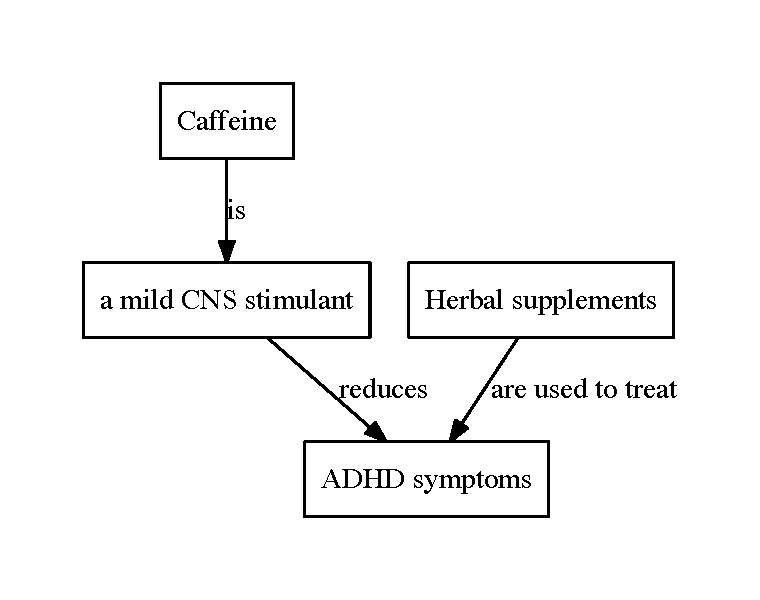
\includegraphics[width=0.5\linewidth]{assets/figures/concept_map.pdf}
\caption{Example of a concept map. The nodes are the concepts. The directed edges connect the concepts to each other and have labels. In this example of a concept map, one could recover sentences from this graph, for example ``Caffeine \textit{is} a mild CNS stimulant". Taken and adapted from: \cite{Falke2017}}
\label{fig:concept_map}
\end{figure}

Concept maps are useful for visualizing concepts and their relation to each other.
Concept maps can be used to quickly explore a given topic and immediately see connections between concepts.
Through the degree of a concept, one can also infer the relative importance of that concept in the underlying text.

By combining different texts of the same topic, one can also create a concept map for the whole topic.
In this case, the concepts are not confined to a single text.
The visualization with concept maps of one or more individual texts therefor enables the non-linear exploration of multiple texts of a topic at the same time.

Since the concepts in a concept map often contain only a small subset of the text, concept maps also summarize the underlying text.
Only relevant concepts and their relation to each other are captured, making concept maps interesting for (multi-document) text summarization.

Another interesting property is that concept maps with its directed edges can be ``unrolled" into text again, enabling conventional text-processing.
Figure \ref{fig:concept_map_linearization} shows an example of such an unrolled concept map.

\begin{figure}[ht!]
	\centering
	\begin{subfigure}[b]{.49\linewidth}
		\centering
		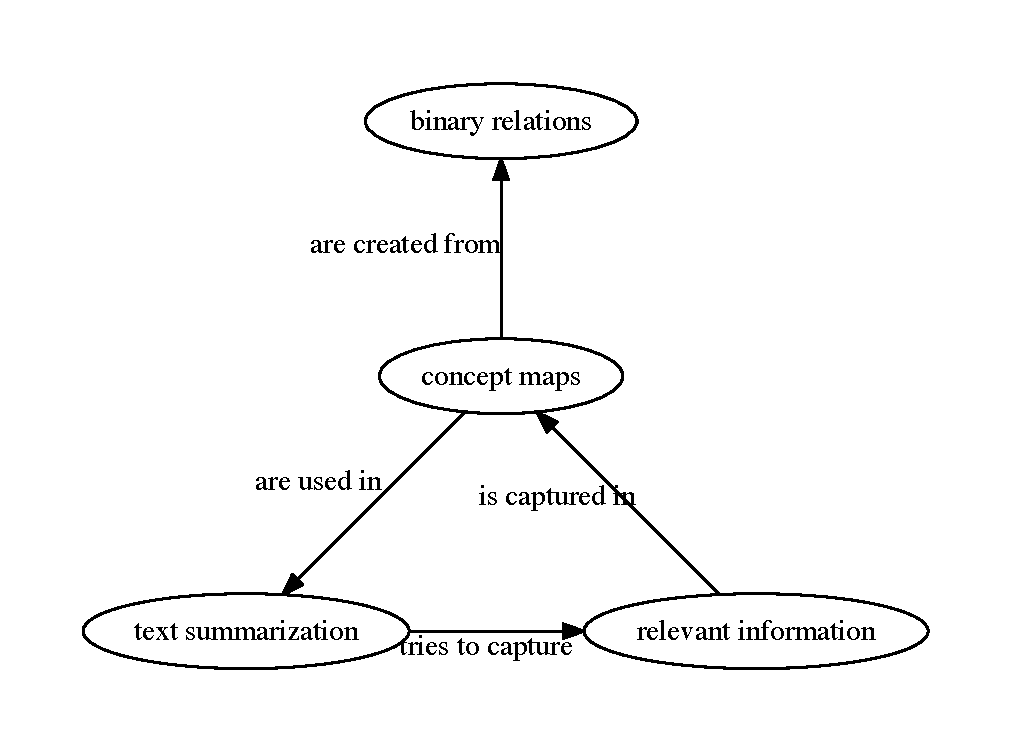
\includegraphics[height=2.2in]{assets/figures/graph_example_linearization.pdf}
		\caption{Concept map}
	\end{subfigure}
	\begin{subfigure}[b]{.49\linewidth}
		\centering
		\noindent\fbox{%
			\parbox{\textwidth}{%
				\textsf{concept maps \enspace\textbf{are used in}\enspace text summarization.
					\\
					concept maps \enspace\textbf{are created from}\enspace binary relations.
					\\
					text summarization \enspace\textbf{tries to capture}\enspace relevant information.
					\\
					relevant information \enspace\textbf{is captured in}\enspace concept maps.
		}}}
		\vspace{0.7in}
		\caption{Extracted sentences}
	\end{subfigure}%
	\caption{Example of a concept map with its linearized version.
		The directed edges with their source- and sink vertices get unrolled into sentences.
		Note that there are as many sentences as there are edges in the original concept map.
		Linearizing a concept map in such a way enables conventional text-processing approaches, eg. extracting word counts with \textit{BoW} then classifying with a \textit{SVM}.}
	\label{fig:concept_map_linearization}
\end{figure}

In Chapter \ref{sec:implementation} we introduce the concept map extraction implementation we used and further explain the steps in creating the concept maps.

\subsubsection{Co-Occurrence Graph}
A co-occurrence graph, or graph-of-words, is generated from a text by creating a graph with all the words of the underlying text as nodes.
There is an edge between two nodes if the labels of the source and target node co-occur in the text.
Two words co-occur when the distance between the words in the text is below a given threshold, the window size.
Co-occurrence graphs can have edge weights corresponding to the counts of the co-occurrence of the words in the text.

Figure \ref{fig:cooccurrence_graphs} shows examples of co-occurrence graphs with different windows sizes.

\begin{figure}[ht!]%
    \centering
    \begin{subfigure}[t]{0.33\linewidth}{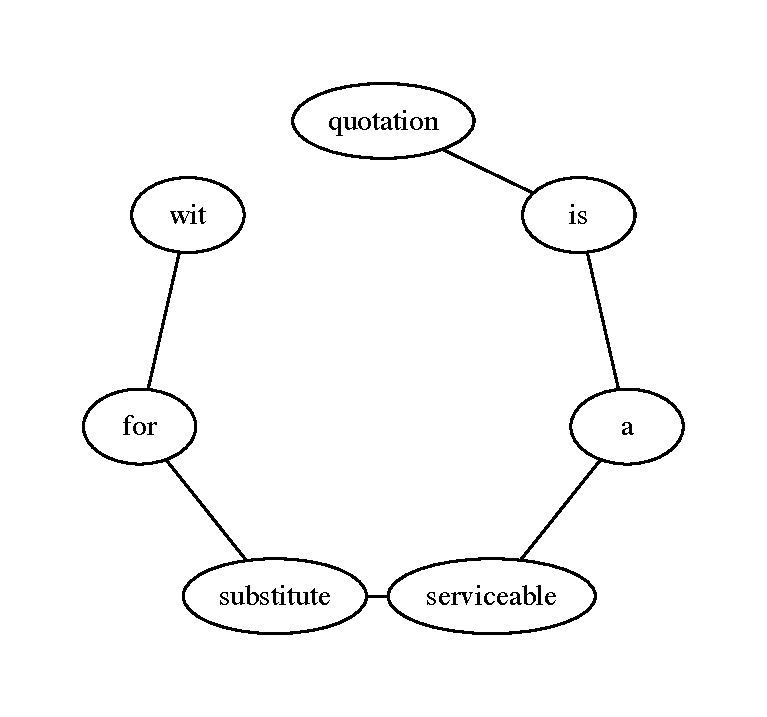
\includegraphics[width=\linewidth]{assets/figures/cooccurrence/window_size_1.pdf}}%
    \caption{Window size: 1}%
    \end{subfigure}
    \begin{subfigure}[t]{0.33\linewidth}{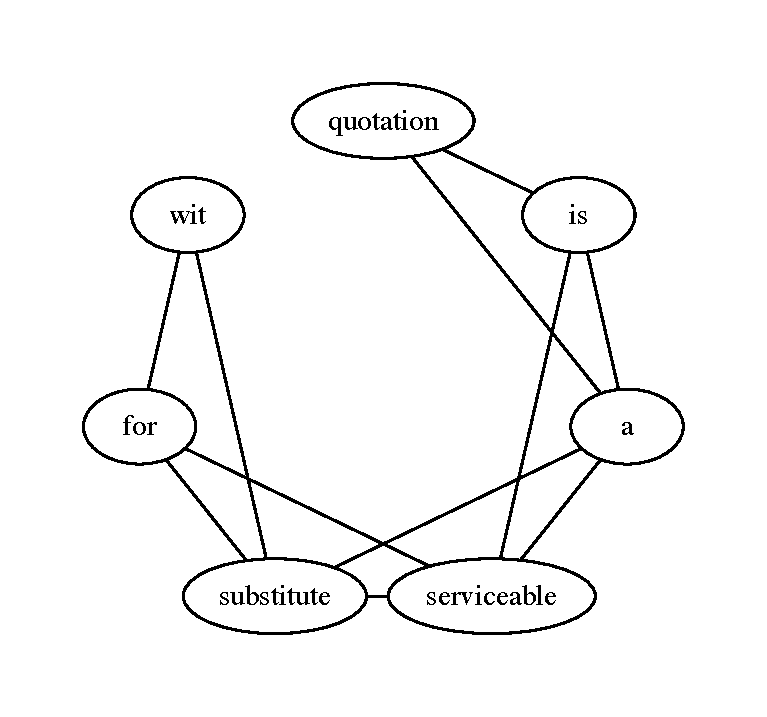
\includegraphics[width=\linewidth]{assets/figures/cooccurrence/window_size_2.pdf}}%
    \caption{Window size: 2}%
    \end{subfigure}
    \begin{subfigure}[t]{0.33\linewidth}{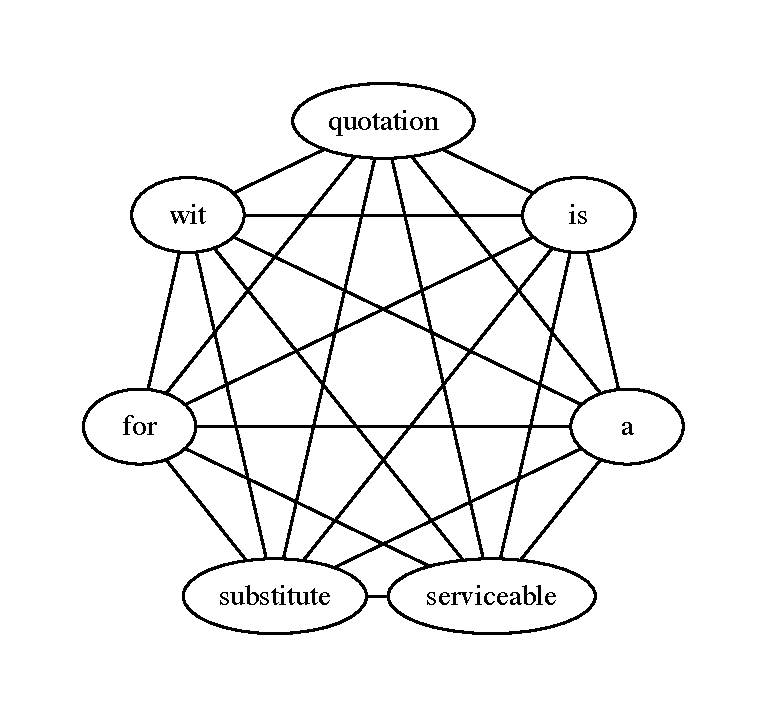
\includegraphics[width=\linewidth]{assets/figures/cooccurrence/window_size_6.pdf}}%
    \caption{Window size: 6}%
    \end{subfigure}
    \caption{Example for co-occurrence graphs. Generated from the sentence: ``Quotation is a serviceable substitute for wit". With increasing window size, the number of edges and therefor the connectedness of the co-occurrence graph also increases.}%
    \label{fig:cooccurrence_graphs}%
\end{figure}

Since co-occurrence graphs not only contain the words of the underlying text but also their co-occurrence, they capture not only the content of the text but also the relation between words of the text.
Therefor they contain structural information about the text.
But, given a co-occurrence graph, it is not possible to recover the underlying text since all information about word-order or sentence structure is omitted.
That said, one could augment co-occurrence graphs by using directed edges and therefor keep the word-order intact.
Yet, even with this augmentation one can not reconstruct the original text.

Because of their similarity to concept maps, we will use co-occurrence maps as a baseline for the graph classification.
It has to be noted that this comparison is not entirely fair since co-occurrence graphs contain all words of the text and there is only a small loss of information.
The concept maps we extracted on the other hand have a far greater compression factor as we will see, ie. they summarize the content more.
For our comparison, we will also not use the edge weights since concept maps do not have edge weights.

\labelsubsection{Graph Kernels}{subsec:graph_kernel}
In most cases, texts and graphs are not of fixed size.
However, most classification algorithms operate on fixed size vectors.
Fortunately, there are several approaches to overcome this problem.
One of the approaches to nevertheless classify non-fixed size objects are so-called kernels.

A kernel is a function $k$ which returns a measure of similarity between two objects:
\begin{equation*}
k: X \times X \rightarrow \mathbb{Q}
\end{equation*}

A kernel function has to be:
\begin{itemize}
    \item{\textit{symmetric}: $k(x, x') = k(x', x)$}
    \item{\textit{non-negative definite}: $\forall x, x': k(x, x') \geq 0$}
\end{itemize}

An interesting property of kernels is that they can be combined easily with symmetric operations, eg. by adding or multiplicating the results of two kernel functions, $k_1$ and $k_2$:

\begin{equation*}
k_{combined}(x, x') = k_1(x, x') \cdot k_2(x, x')
\end{equation*}

One can easily confirm that when $k_1$ and $k_2$ are valid kernels, $k_{combined}$ is also a valid kernel.
This property enables composite kernels to capture multiple means of similarity in one metric.

For example, a simple kernel on two numbers (or vectors) is $k(x, x') = | x \cdot x' |$, where $| \cdot |$ is the absolute value (or a norm).
Another example of a kernel between strings is $k(s, s') = \delta(s = s')$, where $\delta(\cdot)$ is the Kronecker delta. This kernel returns 1 if the two given strings are the same, and 0 if they are different.
Note that both these kernels are indeed valid.
That said, when using kernels in the real world, one can also use non-valid kernel, ie. kernels which are non-symmetric and/or return negative numbers. While such ``kernel" are not strictly valid, they can nevertheless perform good in real-world applications, even better than valid kernels.

Kernels can be used in kernel methods for classification and other tasks.
Prominent examples of kernel methods are the SVM, kernelized PCA and Gaussian Processes.
Later, we will see an example of such kernel methods.

For a subset of kernels, one can also create explicit feature vectors for a given object. In this case, the kernel can be written as an inner product on two fixed-size vectors:

\begin{equation*}
    k(X, X') = \langle \phi(X), \phi(X') \rangle
\end{equation*}

Here, $\phi(X)$ returns a fixed-size vector representation of the object $X$ and is the main part of the kernel.
This $\phi(X)$ can then be used in all vector-based classification algorithms, not only kernel methods.
An example for such a kernel is the string kernel which counts the number of occurrences of words in a given text, then creates a vector representation by giving each word an index in the vector and setting this index to the number of occurrences of that word. The inner product of two of these vector representations then create a kernel.

A graph kernel is simply a kernel that operates on graphs.

Graph kernels that measure the similarity of two graphs are related to the isomorphism test between two graphs.
The graph isomorphism test returns whether two graphs are structurally the same.
In this test, the labels of the vertices and edges are ignored. Otherwise the task would be far easier since one could simply compare the labels and edges of the graphs - when they are both exactly the same, the graphs are the same.
Instead, in the graph isomorphism test one has to find two mappings: one bijective mapping $\psi_{V}: V_1 \mapsto V_2$ from the vertices of the first graph to the vertices of the second graph and another bijective mapping $\psi_{E}: E_1 \mapsto E_2$ with the constraint:

\begin{equation*}
    \forall e = (v_s, v_t) \in E_1:
    \exists e' = (v'_s, v'_t) \in E_2:
    \psi_{E}(e) = e'
    \Rightarrow
    \psi_{V}(v_s) = v'_s
    \land
    \psi_{V}(v_t) = v'_t
\end{equation*}

\todo{Explain constraints for the mapping}

If such a mapping exists, the two graphs are called isomorphic.
While the complexity of the graph isomorphism test is not known yet, it is suspected to lie in P or it may also be NP-complete.
 
One could use the graph isomorphism test, or a variant thereof, to create a graph kernel $k_{isomorphism}$ by returning 1 if the two graphs are isomorphic and 0 otherwise.
Yet, as we noted before, the runtime of the graph isomorphism test is high and also, in the presented version, does not take edge or node labels into account.
We will see other examples of graph kernels in the next paragraphs.
Note that each graph kernel has different strengths and weaknesses, often being subject to a trade-off between accuracy versus compute time.
So, when choosing a suitable kernel, the importance of each aspect of the graphs, eg. labels or structure, has to be assessed.

\paragraph{Gram matrix}
A gram matrix, or kernel matrix, for a given kernel is a matrix $A$ for a set of objects, $D = (x_1, x_2, \ldots, x_n)$ where the entries are the pairwise similarities between all these objects in the dataset:
\begin{equation*}
    A_{i,j} = k(x_i, x_j)
\end{equation*}
So, the entry in the $i$-th row and $j$-th column signifies the similarity of $x_i$ and $x_j$ under the given kernel.

When the explicit feature map $\phi(x)$ for each $x$ is given, one can also construct the gram matrix by stacking these vectors into a matrix $M_{\phi}$ and calculating the product on the transpose
\begin{equation*}
    A = M_{\phi} M_{\phi}^T
\end{equation*}
The gram matrix is symmetric by definition since the underlying kernel is also symmetric, ie. $A_{i,j} = A_{j, i}$.

\paragraph{Graph Kernel Categories}
Several graph kernels have been proposed in the literature.
Categories of graph kernels include kernels based on shortest-paths \cite{Hermansson2015, Borgwardt2005, Nikolentzos2017b}, random-walks \cite{Neuhaus2006a} and subtree patterns\cite{ShervashidzeNINOSHERVASHIDZE2011,Douglas2011,Shervashidze2009,Kersting2013}, to name just a few.

A great number of graph kernels have in common that they first create a decomposition of the graph into sub-structures, for example into subtrees, and then count the occurrences of these sub-structures in the graphs.
The kernels of this kind are sometimes called R-Convolution graph kernels \cite{Namomsa1965a}.
In the next section, we introduce some examples of graph kernels to get a feeling for the possibilities and trade-offs different approaches have.
As mentioned before, any set of valid kernels can be combined easily to form a composite kernel.
So, any of the algorithms we will introduce in the next section can be combined and extended using other kernels.
As we will also see in this next section, graph kernels can be quite diverse and capture different information of the objects they are operating on.
The scope of a graph kernel can therefor also vary widely from only capturing narrow aspects of the graph to actually incorporating the complete graph structure and content.

For a more detailed overview on graph kernels, \cite{Gartner2003a} contains a survey of current graph kernel approaches.

\subsubsection{Examples}
\paragraph{Simple Equality Graph Kernel}
This graph kernel simply compares the nodes and edges of the two graphs and returns whether they are exactly the same:
\begin{equation*}
    k(G_1, G_2) = \delta(V_{G_1} = V_{G_2}) \cdot \delta(E_{G_1} = E_{G_2})
\end{equation*}
This kernel takes both structure and content of the graphs into account. Note that there is no partial similarity. The co-domain of $k$ is $\{0, 1\}$, returning 1 when the graphs are exactly the same and 0 otherwise.
While this is an exact, simple and fast algorithm, in most cases it is not of great use since it depends on exact matches.

\paragraph{Simple Non-Structural Graph Kernel}
Following is an example of a simple kernel which actually discards all structural information about the graph. This graph kernel only operates on the labels of the vertices:
\begin{equation*}
k_{common\_label}(G_1, G_2) = | l(G_1) \cap l(G_2) |
\end{equation*}
where $l(G)$ returns the set of labels for graph $G$.
Therefor, this graph kernel counts the number of common labels of the two graphs. Under this kernel, two graphs are the same when they have the same node labels, completely ignoring the edges.

An extension to this graph kernel is using the Jaccard coefficient instead of simply counting the common node labels:
\begin{equation*}
k_{common\_label\_jaccard}(G_1, G_2) = \frac{| l(G_1) \cap l(G_2) |}{| l(G_1) \cup l(G_2) |}
\end{equation*}
This extension normalizes the function and confines the codomain of $k$ to $[0, 1]$.

\paragraph{Simple Structure-Only Graph Kernel}
An example for a graph kernel which only operates on the structure of the graph, is the following:
\begin{equation*}
k_{simple\_structure}(G_1, G_2) = \langle \phi(G_1), \phi(G_1) \rangle
\end{equation*}
with $\phi(G) = (n_{triangle}(G), n_{rectangle}(G))^T$. Here, $n_{triangle}$ is the number of the triangle subgraphs in $G$ and $n_{rectangle}$ the number of rectangle subgraphs in $G$.
This graph kernel is an example of a kernel where the explicit feature map $\phi(G)$ can be computed directly and completely independent of other graphs.
It is also an example for a R-convolution kernel.

The graphlet kernel is quite similar to this example kernel $k_{simple\_structure}$: instead of counting the number of triangles or rectangles, the graphlet graph kernel counts so-called graphlets.

\todo{Explain graphlets}

\paragraph{Random Walk Graph Kernel}
This kernel does random walks on both graphs and returns the number of matching random walks between the two graphs:
\begin{equation*}
    k(G_1, G_2) = |r(G_1, n, l) \cap r(G_2, n, l)|
\end{equation*}
where $r(G, n, l)$ returns a set of $n$ random walks of length $l$ on graph $G$.
This graph kernel takes both structure and content into account.

\paragraph{Weisfeiler-Lehman Graph Kernel}
The Weisfeiler-Lehman graph kernel is also a kernel that works by counting common sub-structures on two graphs.
Here, the sub-structures are subtrees starting from each vertex.
In each iteration $i$ with $0 < i < h$ for a given number of iterations $h$ , or until convergence, the WL graph kernel relabels the vertices of the two given graphs.
This relabeling is also called recoloring or color refinement.

The WL graph kernel relabels a vertex $v$ by concatenating two components:
\begin{enumerate}
    \item{the current label of the vertex: $\pi_{i-1}(v)$}
    \item{the sorted labels of the neighbourhood: $\{ \pi_{i-1}(v') | v' \in n(v) \}$}
\end{enumerate}
where $\pi_{i}$ is the labeling function for iteration $i$ with $\pi_0 = \pi$.
The resulting new label of $v$ is the sequence $(\pi_{i-1}(v), \pi_{i-1}(v_{neighbour,1}), \dots , \pi_{i-1}(v_{neighbour,n}))$.
After the iteration, a new labeling function is created accordingly: $\pi_i(v)$ now returns to the new label of $v$.
So, for each iteration, a node gets the same label as another node if they have the same label and neighbourhood.
For the first iteration, the labels of a node consist of the immediate neighbourhood.
In the next iteration, the label of a node than encodes the neighbourhood of the neighbourhood, ie. 

The Weisfeiler-Lehman graph kernel has been shown to achieve state-of-the-art performance on several datasets and applications.
It takes into account both content and structure, while also performing good in terms of compute-time.

\todo{Complexity? $\mathcal{O}(hm)$, where $h$ is the number of iterations and $m$ is the number of edges in the dataset.}

It has to be noted that the Weisfeiler-Lehman does not use edge labels by default, but can be extended to do so.
There are also several other extensions to the Weisfeiler-Lehman kernel in the literature.
One example of such an extension reduces the space requirement of the algorithm by ``compressing" the labels after each iterations, ie. by giving each composite label a unique and shorter label.

In Figure \ref{fig:wl_example} we show an example of one WL iteration with label compression.

In this work we will use a variant of the WL graph kernel called \textit{fast\_wl} which was introduced in \cite{Kersting2013}.
This variant improves the run-time of the plain Weisfeiler-Lehman kernel by cleverly creating a hash of the neighbourhood to create the new coloring for the graph.
The results are exactly the same as with the plain Weisfeiler-Lehman kernel yet the calculation of the new labels is significantly faster.
Our implementation also uses label compression, explained in Figure \ref{fig:wl_example}, to further speed up the calculation and assigning integer indices to the new labels, therefore enabling the creation of explicit feature maps $\phi(G)$.

\begin{figure}[ht]
  \centering
  \begin{subfigure}[t]{0.33\linewidth}
  {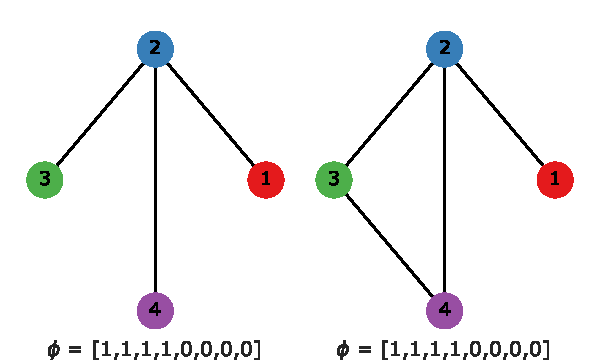
\includegraphics[width=\linewidth]{assets/figures/wl_example/wl_iteration_0.pdf}\label{fig:wl_example_0}}
  \caption{Initial graphs}
  \end{subfigure}
  \begin{subfigure}[t]{0.33\linewidth}
  {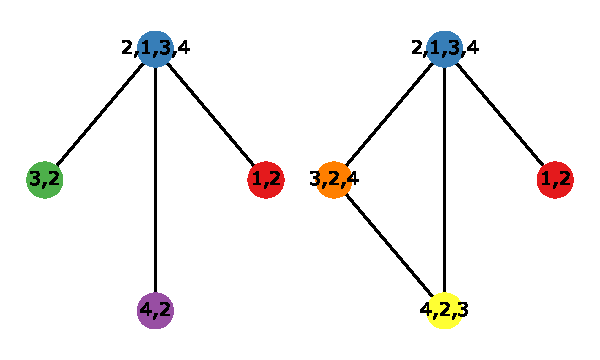
\includegraphics[width=\linewidth]{assets/figures/wl_example/wl_iteration_1_stage_0_recolored}\label{fig:wl_example_1}}
  \caption{After relabeling}
  \end{subfigure}
  \begin{subfigure}[t]{0.33\linewidth}
  {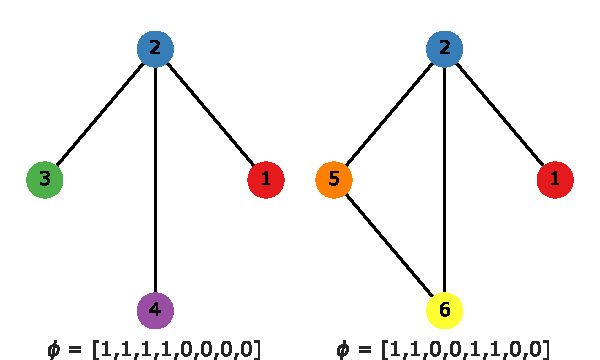
\includegraphics[width=\linewidth]{assets/figures/wl_example/wl_iteration_1_stage_1_compressed.pdf}\label{fig:wl_example_2}}
  \caption{After label compression}
  \end{subfigure}
  \caption{Weisfeiler Lehman algorithm example. This examples shows one WL iteration with two graphs. The initial graphs are shown in \textbf{(a)}. The first step of the iteration is relabeling the graph vertices by concatenating each node label with its sorted neighbourhood labels. The finished relabeled graph is shown in \textbf{(b)}. As an extension to the plain Weisfeiler-Lehman algorithm, we also show the label compression step where the long labels, consisting of the node label and its neighbourhood labels, get compressed into a smaller label by assigning each unique label a new number. Same labels in different graphs get the same new label. The result of this step is shown in \textbf{(c)}. Under \textbf{(a)} and \textbf{(c)} we also added the feature maps $\phi{}$ for the graphs. Each entry in the vector corresponds to a label. If a vector entry is 1, it means that the corresponding label is present in the given graph. The inner product on the vectors of the graphs is the value of the Weisfeiler-Lehman graph kernel for these two graphs.
  In this case, the similarity before the iteration would be $\langle \phi(G_1), \phi(G_2) \rangle = \langle [1, 1, 1, 1, 0, 0, 0, 0], [1, 1, 1, 1, 0, 0, 0, 0] \rangle = 4$. After the relabeling, the value of the inner product is $2$.
  Before doing the WL iteration, the inner product on the feature maps simply returns the number of common labels. After the first iteration, the neighbourhood of each node and therefor the structure of the graph is also reflected in the feature map - resulting in a lower similarity in out example.
  Please note that these feature vectors are specific to these two graphs and their labels. The dimension of the vector corresponds to the sum of the number of vertices in the two graphs.}\label{fig:wl_example}
\end{figure}

\subsubsection{Kernel Methods and Kernel trick}
We have seen that a kernel can be used to calculate a measure of similarity between two objects, eg. graphs.
Some kernels can be expressed as an inner product $k(X, X') = \langle \phi(X), \phi(X') \rangle$ on two (implicit) vector representations of the objects $X$ and $X'$.
In this case, the vector representations $\phi(X)$ can be used in conventional classification algorithms.
Yet, calculating these representations is not always possible or feasible since the dimension of such a representation is quite high.
There is another approach for classification (and regression), the aforementioned kernel methods.
Kernel methods operate directly with the kernel values and do not use the implicit feature representations $\phi(X)$.
Instead, kernel methods use the similarities $k(X, X')$ directly.

One popular example of a kernel method is the Support Vector Machine, or SVM.
The SVM is able to use both vector representations of elements in the dataset or the pairwise similarities, the gram matrix, between them.
At training time, the gram matrix $A$ of all objects in the training set, $d_{train} = \{X_1, X_2, \ldots, X_n\}$, is calculated.
This gram matrix $A$ and the corresponding classes then get fed into the SVM which fits its coefficients to them.
After training, to predict the label for a given instance $X_{test}$, the pairwise similarities of t$X_{test}$ and all training examples are calculated, resulting in a vector $v = (k(X_{test}, X_1), k(X_{test}, X_2), \ldots, k(X_{test}, X\_n))$.
This vector $v$ is then fed into the SVM which predicts the label for $X_{test}$.
Note that this kernel method approach does not use explicit feature maps of the instances, only their pairwise similarities.
This feature of not needing to calculate the explicit feature map $\phi$ is called kernel trick.
It enables linear models, such as the SVM, to solve non-linear separable problems.

In our work, we will use both the kernelized version of the SVM, ie. learning with a gram matrix, as well as the version using an explicit feature map $\phi$.


\labelsubsection{Graph Kernel Based Text Classification}{subsec:graph_kernel_based_text_classification}
In this section, we will introduce related work and briefly recap the history of the field.

\todo{How did the field evolve?}
\todo{Hint related tasks}
\todo{What is the most related work, how do they differ from our approach}
\todo{Relate the other work to the new approach and work out their differences/results}
\todo{Other approaches to graph classification}
\todo{Mention other graphs}

\paragraph{``Shortest-Path Graph Kernels for Document Similarity" \cite{Nikolentzos2017a}}
The most similar and recent work to our approach that we found was \cite{Nikolentzos2017a}. In this work, the authors first create co-occurrence graphs out of the text. Next, they create the gram matrix for the graphs with their own graph kernel and use a SVM to classify them.

Their graph kernel is a combination of two sub-kernels:
\begin{enumerate}
    \item{\textit{Simple label matching}: the number of matching node labels are compared between the two graphs}
    \item{\textit{Shortest path}: generate a shortest-path graph, then compare the edges}
\end{enumerate}
Note that the simple label matching sub-kernel does not take the structure into account, while the second sub-kernel actually uses both.
Both sub-kernels return a number which is added to produce the final value of the kernel.

The shortest path sub-kernel works as follows:
\begin{enumerate}
    \item{Generate shortest-path graphs for the two given graphs: The shortest path graph of a given graph has the same nodes.
    The edges are added by calculating the shortest paths between all pairs of nodes in the original graph. An edge is added between two nodes in the shortest path graph if the shortest path length between these nodes in the original graph is below a given parameter $d$. The edge also gets a weight assigned, which is $\frac{1}{d}$}
    \item{Count the number of same edges in the both graphs: when two edges are the same, add the product of their edge weights to the similarity}
\end{enumerate}

\todo{Mention that they did NOT perform experiments to differentiate the performance of the subkernels! My guess is that most of the performance comes from the simple-set matching subkernel.}
\todo{Note that the shortest-path sub-kernel does not actually add a lot of performance?}
\todo{Why is this approach different to ours? Co-occurrence vs. concept map}

\paragraph{``Text Categorization as a Graph Classification Problem" \cite{Rousseau2015a}}
In this paper, the authors generate co-occurrence graphs out of different text classification datasets.
To classify the graphs, they introduce their own graph kernel which is also an instance of the aforementioned kernels that count the number of occurrences of sub-structures.
In this case, the sub-structures this kernel counts are frequent subgraphs, ie. subgraphs that occur frequently in the graphs of the dataset.
To get a set of most-frequent subgraphs in the dataset, they develop their own approach, using depth-first search and a labelling function for graphs that enables finding frequent subgraphs efficiently.
After extracting the sub-graphs from the dataset this way, they only retain subgraphs which occur more often in the dataset than some defined parameter, the support value.
This significantly reduces the number of considered sub-graphs since most subgraphs occur quite infrequently.
This extension is indeed needed since the number of possible sub-graphs grows super-linear with the number of nodes/edges and can render the subsequent counting of the sub-graphs in the dataset infeasible.
Also, considering all possible subgraphs in all graphs in the dataset would not only require significant computational resources but would also result in sparse feature vectors since most sub-graphs occur infrequently.
This, in turn, would harden the classifier training problem.

As another measure to lower the runtime complexity of their algorithm, they also first extract the main core of each co-occurrence graph and only extract sub-graphs from them, not from the whole graphs.
A $k$-core is a subgraph $G_k$ of graph $G$ where all vertices have a degree greater or equal to $k$. The main core of a graph is the $k$-core with the highest possible $k$.
Thus the main core is the most connected subgraph of graph $G$, which includes only the most ``important" vertices and their edges to each other.

So, after extracting the main-core of each co-occurrence graph and determining the set of most-frequent sub-graphs in the dataset, they count the occurrences of the most-frequent sub-graphs for each graph in the dataset.
This results in feature maps $\phi_i$ which contain the counts of each most-frequent sub-graph per co-occurrence graph.
These feature vectors together with the labels are then used to train a SVM and are used to subsequently predict new instances by creating their feature maps and then predicting the label with this trained SVM.

The authors evaluated the classification performance of their approach on several datasets, namely the WebKB corpus, a subset of the reuters-21578 corpus (named R8), the ling-spam dataset and a corpus of Amazon reviews.
In our work, we also use these and other datasets. In later sections, we will introduce then more thoroughly.

In the paper, the authors argue that only retaining the main-core does not greatly damage the classification performance, yet it significantly reduces the compute time.
They also stress the importance of choosing an adequate support value for the sub-graph mining, mentioning the trade-off between performance and considered features. The process of choosing an adequate support value can be done unsupervised and gets treated similar to hyperparameter tuning of, for example, SVM hyperparameters.

This paper is quite similar to our approach since it also poses the text classification task as a graph classification task. Yet, they consider only one type of graph, the co-occurrence graph of the underlying texts.
Also, they do not evaluate the effect of combining text- and graph features.
That said, they provide interesting comparisons of text- and graph based approaches, pointing out the similarity of n-grams with the relationships which are captured in co-occurrence graphs.

\paragraph{``Concept Graph Preserving Semantic Relationship for Biomedical Text Categorization" \cite{Gulrandhe2015}}
Graphs: extracted keywords/concepts (POS tagger, only nouns), mapping of concepts to UMLS database, extraction of relationship between them.

Nodes are get 4 different weight components: tf, idf, connectivity, \#connected components.

Kernel: number of shared edges

No results


\paragraph{``Text classification using Semantic Information and Graph Kernels" \cite{???}}
In this paper, the text classification task is also converted into a graph classification task.
The authors create a graph of the underlying text by extracting so-called \underline{D}iscourse \underline{R}epresentation \underline{S}tructures, or DRS, which capture the semantic relationships in the sentences of the underlying text.
A DRS consists of two parts, namely a set discourse referents, or entities, and conditions on these entities.
The example given in the paper constructs the DRS for the sentence ``He throws the ball", which results in the DRS with the entities $\{\text{He}, \text{ball}, \text{throws}\}$ which get renamed to $\{x1, x2, x3\}$.
The conditions then define the meaning or relationship of the items. In the given example the DRS conditions are $\{\text{male}(x1), \text{ball}(x2), \text{throws}(x3), \text{event}(x3), \text{agent}(x3, x1), \text{patient}(x3, x2)\}$.

\todo{How to cite this example?}

To construct a graph from the extracted DRS', the entities become vertices and the conditions become edges between them.
A unary condition on a vertex, for instance $\text{male}(x1)$, becomes a loop for the node $x1$.
Conditions on two entities become directed edges, going from the entity of the first argument to the second condition argument, for example the condition $\text{agent}(x3, x1)$ creates a node from $x3$ to $x1$.
This results in a graph which captures the semantic relationship between the entities of the underlying graph.
Note that edge node labels, or entities, are not as important as the edges , or conditions, between them.
This is accounted for in the kernel the authors use in the next step.
Also note, that the process of creating a DRS graph for a given text is independent of other texts and can easily be parallized.

After constructing DRS graphs for all texts in the dataset, the authors use a variant of a random-walk kernel, customized to capture the importance of the edges instead of the nodes.
In the plain random-walk kernel, random walks are done on the two graphs, $G$ and $G'$ and the counts of equal random walks are counted, resulting in a measure of similarity between these two graphs. The higher the count of equal random walks, the higher the similarity.
The equality of two walks is determined by comparing the labels of the visited nodes.
In the case of DRS graphs, this would not yield a good kernel since the labels of the nodes are placeholders, ie. two vertices with the same label, for example $x1$, can correspond to totally different entities.
So, the standard definition of walk equality can not be used in the case of DRS graphs.
Instead, the authors introduce an approach which, for a given node $v_1$ of graph $G$, returns an ``equal" node $v_2$ in graph $G'$ that has similar edge \textbf{labels}.
This enables the random-walk graph kernel to ``merge" nodes with different node labels, that is placeholder like $x1$, on the two graphs, thus enabling random walks with meaningful node equality in the case of the DRS graphs.
After extracting the gram matrix of the DRS graphs with this extended random-walk graph kernel, the authors then use a SVM to evaluate their approach on the \textit{reuters-21578} dataset.
They use only a subset of 50 texts in the five most frequent classes of the dataset as their corpus. Then they create the DRS graphs for these texts and randomly select 25 of each class to create a gram matrix.
This gram matrix then gets used to train a one-versus-one SVM classifier. So, they do binary classification and present the results of the performance of the pairs of the 5 classes they considered.
The authors explain the reason for this small number of considered documents and classes by mentioning the runtime complexity of their approach, most notably the runtime complexity of the random-walk kernel.
They also acknowledge that they do not provide baseline results or comparisons between different approaches to text-classification or results with other graph kernels.

That said, this work is also similar to our approach in the sense that they also use graphs representations of texts to classify.

\todo{Maybe create similar kernel which does link prediction by defining edge equality through similar source/destination node labels?}

\paragraph{``Deep Graph Kernels" \cite{Yanardag2015}}
In this paper, the authors introduce an extension for existing kernels for which the explicit feature map $\phi$ can be calculated.
When calculating the kernel
\begin{equation*}
k(G, G') = \phi^T(G) \cdot \phi(G')
\end{equation*}
they add a weighting matrix $M$
\begin{equation*}
k(G, G') = \phi^T(G) \cdot M \cdot \phi(G')
\end{equation*}

The intuition here is that each vector entry of $\phi(G)$ corresponds to the count of some substructure of $G$ and that these substructures are not independent of each other, ie. they can be similar to each other.
Yet when calculating the plain kernel only exact matches of substructures in the two graphs are considered.
For instances, suppose substructure $g_1$ is similar to another substructure $g_2$ and substructure $g_1$ is only present in $G$ and not in $G'$, conversely substructure $g_2$ is only present in $G'$ and not in $G$.
Suppose some kernel $k$ would construct $\phi_k(G)$ by counting the occurrences of $g_1$ and $g_2$, so $\phi_k(G) = (n_{g_1}(G), n_{g_2}(G))$ where $n_{g_i}(G)$ counts the occurrence of substructure $g_i$ in $G$.
In the above example, $\phi_k(G_1) = (1, 0)$ and $\phi_k(G_2) = (0, 1)$. When calculating $k(G, G') = \phi_k^T(G) \cdot \phi_k(G') $ the similarity under the kernel would equal 0, therefore ignoring the similarity of substructure $g_1$ and $g_2$.
The proposed extension to the kernel aims to address this issue by using embeddings for the substructures to identify the similarity of substructures and then allowing ``partial" instead of only exact matches.
In the above example, the new $\phi_{new}(G)$ would not be $(1, 0)$ but $(1, i)$ and $\phi_{new}(G') = (i, 1)$ with some $i > 0$.
In our example, the aforementioned matrix $M$ would be
\begin{align*}
M = \begin{bmatrix}
1 & i \\
i & 1
\end{bmatrix}
\end{align*}

In this case, when calculating the kernel for these two graphs, the similarity would be $(1, 0)^T \cdot M \cdot (0, 1) = (1, 0)^T \cdot (i, 1) = i$ instead of $(0, 1)^T \cdot (1, 0) = 0$.
So, the augmented kernel between these graphs would actually capture the similarity of substructures instead of only using exact matches of them.

The authors then introduce two ways to create the matrix $M$ for a kernel, namely by creating it by hand using a measure of similarity between the substructures or by learning the embeddings with an approach similar to the \textit{word2vec} algorithm.
In both cases, the matrix $M$ aims to encode the similarities of the substructures.

The authors report an improvement of classification scores for several real-world datasets, comparing the scores of the plain version of a kernel with their augmented version.


\todo{How does this approach differ from ours?}
  \refsection{Evaluation}{sec:evaluation}
  \todo[inline]{Explain the used metrics and how they relate to hypothesis}
\todo[inline]{Introduce the baselines, explain how they relate to the hypothesis, why they - are chosen, how they differ}
\todo[inline]{Explain methodology, why the chosen metric really captures the problem at - hand}
\todo[inline]{Work out differences of graph types, find similarities across datasets}
\todo[inline]{Provide the questions that are relevant for the hypothesis}
\todo[inline]{Answer these questions through metrics/results}

\todo[inline]{What is the best kernel for concept map classification?}
\todo[inline]{Extensions to WL?}


In order to test the hypothesis, we first derive a number of questions from the hypothesis.
We will also often compare the results on these questions for concept maps to co-occurrence graphs to find differences. While the comparison to co-occurrence graphs is interesting by itself, it is not entirely fair since co-occurrence graphs have far more nodes than concept maps.
Nevertheless, co-occurrence graphs capture the words of a text completely.

In the next chapter, we will give the results to the questions we posed in this chapter and also discuss their significance to the hypothesis.

\labelsubsection{Experiments}{subsec:experiments}
\todo[inline]{Test the hypothesis}
\todo[inline]{Tables with results}
\todo[inline]{Mention difficulties and possible solutions}
\todo[inline]{Add runtime analysis}

\subquestion{How diverse is the structure of the concept maps?}{question:structure_diversity}
When the structure of the graphs is mostly homogeneous or the structural differences are not distinct between graphs of different classes, the structure by itself will most likely not contribute to the classification performance.
When comparing the graph similarity under some graph kernel, the graphs of a given class should be distinguishable from the graphs of the other classes.

To explore the variance in the structure of concept maps, we look at the following metrics:
\begin{enumerate}
    \item{Histogram of the number of connected components}
    \item{Histogram of the size of connected components}
    \item{Average node/edge ratio}
\end{enumerate}

All these methods aim to find out the diversity of the connectedness of concept maps. There a lot of other metrics, but as we will see later on these metrics suffice to get a good picture about the structure of the concept maps.

\subquestion{How important is the structure of concept maps compared to the content?}{question:importance_structure}
Another important question is the relative importance of the structure compared to the content, or the labels.
For this we compare the results of different graph kernels that use \textbf{(a)} only content and \textbf{(b)} only structure and \textbf{(c)} both content and structure.

For the content-only kernel, we will simply count the number of occurrences of labels in the graphs and essentially create a bag-of-words representation of the graph. The kernel then creates the similarity score by calculating the inner product on these vector representations, effectively counting the number of common labels.

For the structure-only kernel, we will use a modified version of the Weisfeiler-Lehman kernel: before executing the WL kernel on the graphs, we first discard all labels on the graph. All nodes of all graphs get the same label. This way, only the structure gets used for the similarity score.

For the structure-and-content kernel, we use the plain Weisfeiler-Lehman graph kernel. We also added an extension to the kernel by using node weights as weights for the labels. We first extracted a weight for each node by calculating the node degree.
We added this extension to give additional weight to label matches of nodes with a greater number of neighbours, ie. higher degree, since matches with a greater neighbourhood are far less often.
Instead of the degree, one could also use another metric like PageRank and using the resulting node weights.

\todo[inline]{Using node weights is a trade-off: giving the nodes more weight when they are more connect implies that words that occur often have a high importance!}

\subquestion{How does the classification results of co-occurrence graphs compare to concept maps?}{question:comparison_coo}
For this question, we compare the classification results for concept maps and co-occurrence graphs. As noted before, this comparison is slightly unfair since co-occurrence graphs have far more content than concept maps.
Nevertheless, it is an interesting baseline for graph-based text-classification.

\subquestion{How does the classification performance with concept maps compare to non-structural, text-based approaches?}{question:comparison_text}
Here we test the classification performance of graph-based classification directly with the performance of text-only approaches.

\subquestion{How useful are the concept maps combined with text classification?}{question:comparison_combined}
When concept maps indeed have a structure that is useful for classification and which is not captured by text-only approaches, the classification performance should increase when combining graph- and text based approaches.
We test the performance of the combined text- and graph features by concatenating the vectors of both approaches and then training a classifier with these vectors.
We also compare the results with both text-only and graph-only approaches.

\subsubsection{Baselines}
\paragraph{Preprocessing}
Before creating the vector representations of the text documents or the creation of the co-occurrence graphs and concept maps, we first pre-process the plain text by

\begin{itemize}
\item{lowercasing the text,}
\item{removing non-printable characters,}
\item{replacing numbers with a \textit{NUMBER} placeholder,}
\item{replacing tabs and newlines with a space,}
\item{and normalizing the whitespace (eg. replacing multiple spaces with a single space)}
\end{itemize}
These pre-processing steps are similar to the pre-processing done in \cite{Cachopo2007}.

\paragraph{Text-based representations}
For the text classification pipeline, we used two different vectorization algorithms, namely
\begin{itemize}
\item{Bag Of Words (BoW): this vectorizer simply gathers all words in the corpus and creates a mapping between words and indices (ids). Then it creates a vector representation for each text so that the i-th vector component  is the count of the corresponding word in the text. Ie. $i$ is the index of the word in the mapping.}
\item{Term-Frequency-Inverse-Document-Frequency (TfIdf): this approach is similar to BoW. Instead of using only the counts of a word in the text, this approach also incorporates the term frequency and the inverse document frequency of the words to the vector representation (see below).}
\end{itemize}
Both approaches can also be extended by not only utilizing single words (unigrams) but n-grams, too. A word n-gram consists of $n$ words that appear consecutively in the text.
For example, the sentence ``This is a sentence." has the following 2-grams, or bigrams: $\{ (This, is), (is, a), (a, sentence) \}$.
For our purposes, we looked at n-grams of lengths (1), (1, 2) and (2).
Note that word n-grams do not take word inversion into account, ie. the bigram (a, b) is not the same as (b, a).

\todo[inline]{Explain why we used these ranges of n-grams}
\todo[inline]{Explain tfidf}

\paragraph{Graph-based representations}
To compare the performance of concept maps with other graphs, we generated co-occurrence graphs with window sizes of $\{1, 2\}$.

\todo[inline]{Co-occurrence and concept maps}
\todo[inline]{Mention filtering by nouns}
\todo[inline]{Window sizes}
\todo[inline]{Mention Tobias' code for generating the concept maps}

\begin{figure}[ht]
\centering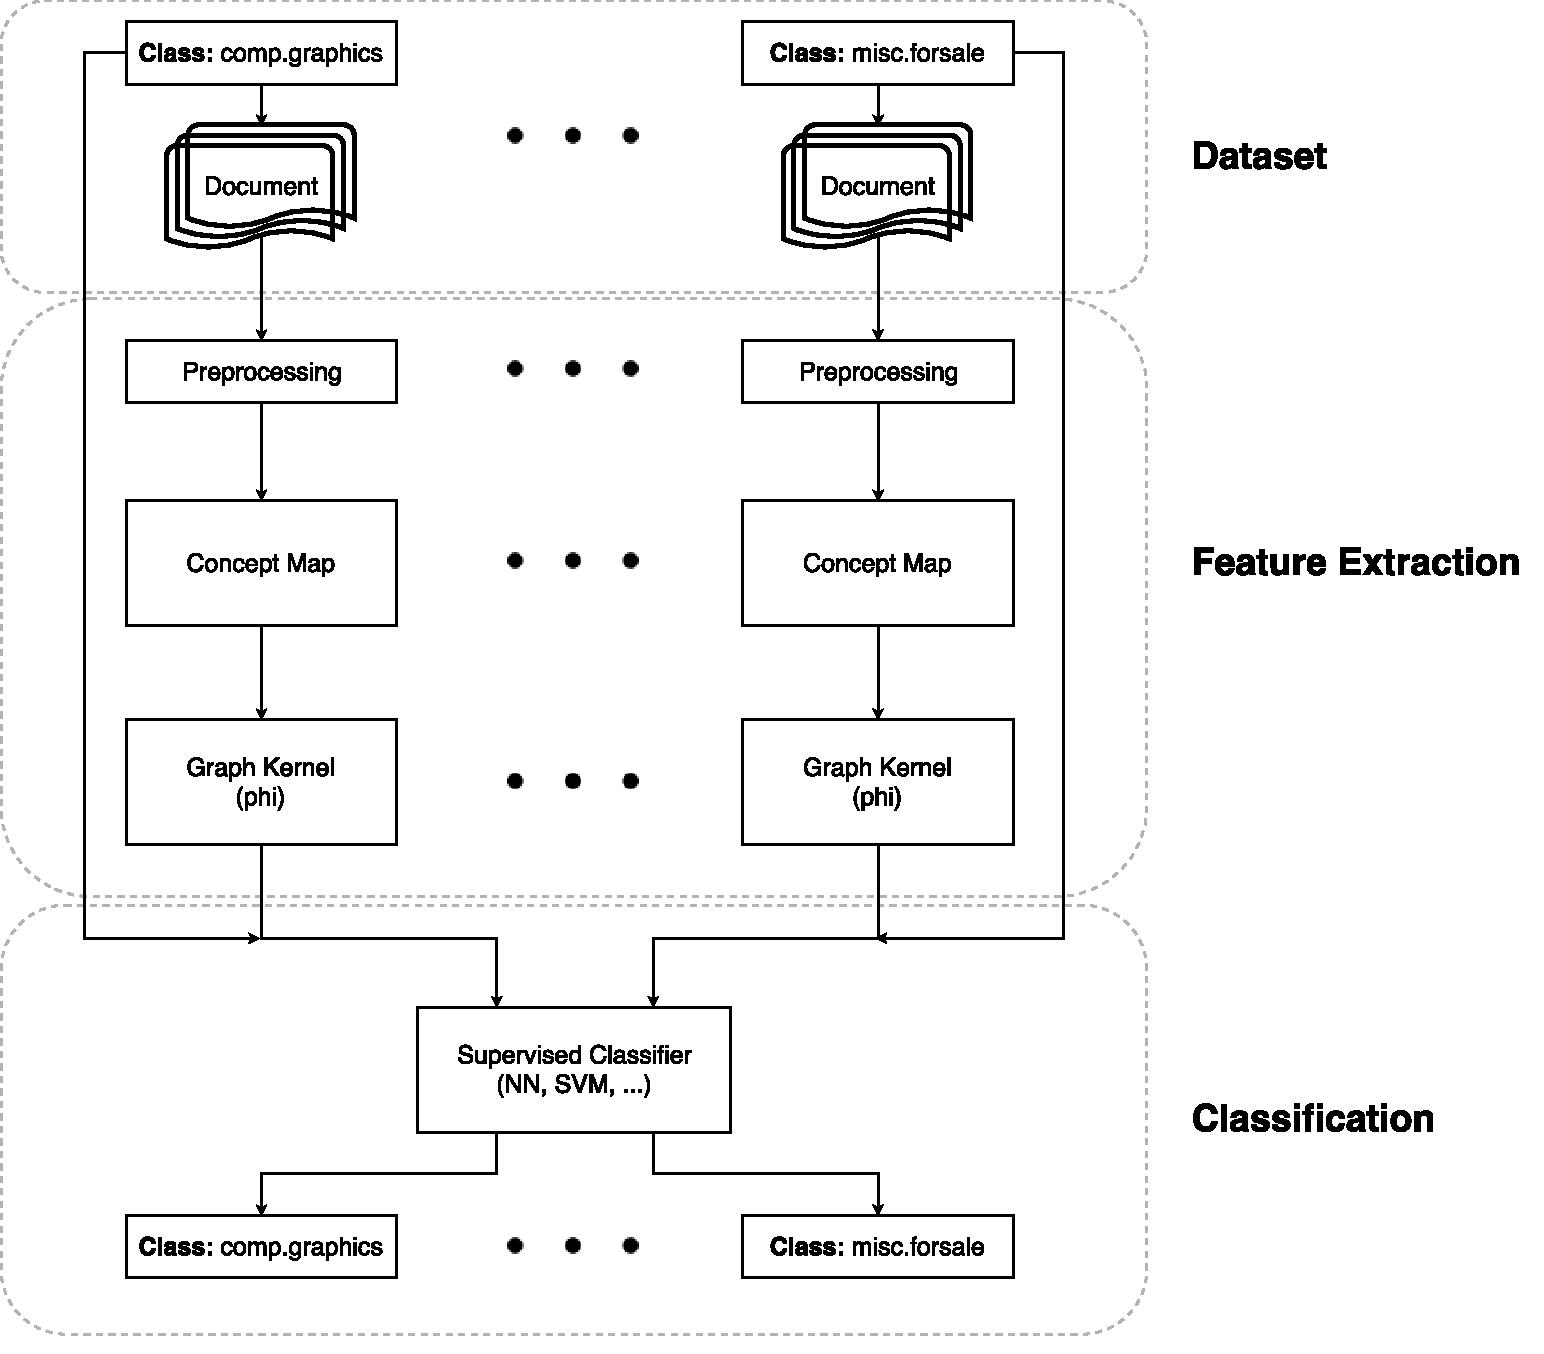
\includegraphics[width=0.6\linewidth]{assets/figures/approach.pdf}
\caption{Graph kernel based classification pipeline.}
\end{figure}
\todo[inline]{Add diagram for gram-matrix based classification.}

\labelsubsection{Datasets}{subsec:datasets}
\todo[inline]{A script to download all datasets is also provided alongside the other code}

\paragraph{ling-spam}
The Ling-Spam dataset was created by Ion Androutsopoulos et al. \cite{Androutsopoulos2000}.
The corpus contains the texts, which are categorized as ``spam" and ``no spam". For this work, we used the version which can be downloaded from here\footnote{\url{http://csmining.org/index.php/ling-spam-datasets.html}}.

\paragraph{ng20}
The 20 Newsgroup corpus \cite{Lang} consists of posts from an internet forum. They are labeled with 20 different classes, corresponding to the topic they have been posted on. The texts are mostly informal and consist of discussions between users of the forum.
For this dataset, as an additional pre-processing step, we remove the headers and footers from the documents.

While the classes are nearly evenly distributed, some classes are highly correlated. This adds an additional difficulty to the task.

\todo[inline]{Explain correlation more throughly}

\paragraph{reuters-21578}
\footnote{\url{http://www.nltk.org/book/ch02.html#reuters-corpus}}
\todo[inline]{Documents came from Reuters newswire in 1987.}

\paragraph{r8}
This dataset is a subset of the \textit{reuters-21578} dataset.
It consists of the 8 most frequent classes of the \textit{reuters-21578} dataset, ie. the 8 classes with the most documents.

\paragraph{review\_polarity}
\cite{Pang2004}.
\footnote{\url{http://www.cs.cornell.edu/people/pabo/movie-review-data/review_polarity.tar.gz}}

\paragraph{rotten\_imdb}
\cite{Pang2004}.
\footnote{\url{http://www.cs.cornell.edu/people/pabo/movie-review-data/rotten_imdb.tar.gz}}

\paragraph{tagmynews}
\footnote{\url{http://acube.di.unipi.it/repo/news.gz}}

\paragraph{webkb}
\footnote{\url{http://www.cs.cmu.edu/afs/cs/project/theo-20/www/data/}}

\begin{figure}[ht]
\centering
\begin{tabular}{lrrrr}
{} &  \# docs &  \# classes &  median \#words/doc &  \#uniq. words/\#words \\
\midrule
ling-spam       & 18846 & 20 & 277 & 0.20 \\
ng20            & 2893 & 2 & 79 & 0.22 \\
reuters-21578   & 18846 & 20 & 94 & 0.07 \\
review\_polarity & 13328 & 90 & 589 & 0.16 \\
rotten\_imdb     & 2000 & 2 & 19 & 0.34 \\
tagmynews       & 10000 & 2 & 24 & 0.11 \\
webkb           & 32600 & 7 & 158 & 0.15 \\
\bottomrule
\end{tabular}
\caption{Dataset statistics}
\end{figure}

\labelsubsection{Methods}{subsec:methods}

\subsubsection{Cross-Validation}
For all the classification tasks we used train-/validation- and test sets.
The split is done as follows: 85\% for train- and validation set together and 15\% for the validation set.
We then use stratified k-fold cross-validation to further split the train- and validation set. In our case, we used $k = 3$, meaning that $\frac{2}{3}$ of the dataset is used for training, and the rest for validation.
The stratification ensures that the class distribution in the train set is (nearly) the same as in the validation set.

\todo[inline]{Hold-out set!}

\subsubsection{Metrics}
We evaluated a number of metrics for each classification task, namely: 
recall, precision, accuracy and the F1-score. We mostly focus on the F1-score since it captures the overall performance of classification algorithms.

\subsubsection{Significance tests}
When comparing two models we used the permutation test, or exact test, to test the significance of the difference in performance of these two approaches.
The permutation test tests whether the observed difference of the performances of the two approaches is the product of chance.
The test only returns a probability for observing a given performance difference. The test does not give a definite answer whether the difference was due to chance.
When the probability of observing the difference by chance is below a given threshold, we say that the test shows that the approaches really differ in their performance.

\todo[inline]{What confidence interval did we choose?}

\begin{figure}[ht]
  \subfloat[True labels]{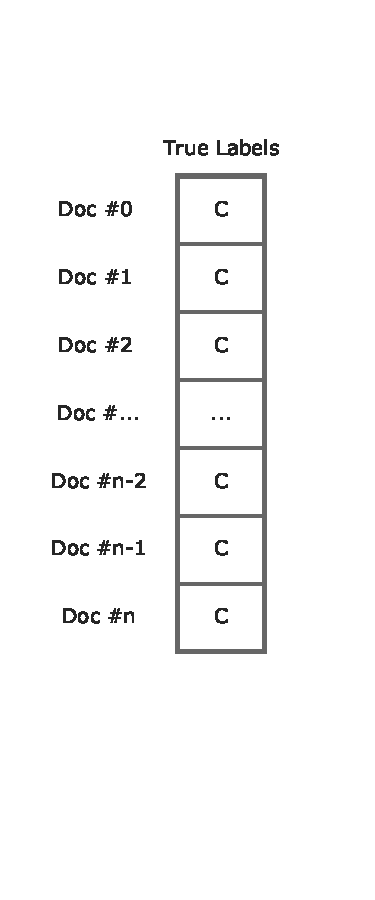
\includegraphics[width=0.19\textwidth]{assets/figures/permutation_test/true_labels.pdf}\label{fig:permutation_test_true}}
  \hfill
  \subfloat[Predictions]{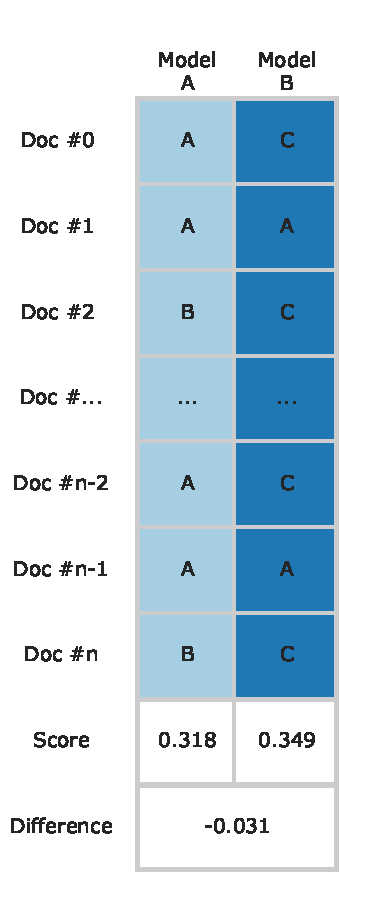
\includegraphics[width=0.17\textwidth]{assets/figures/permutation_test/initial_predictions.pdf}\label{fig:permutation_test_model_predictions}}
  \hfill
  \subfloat[Samples]{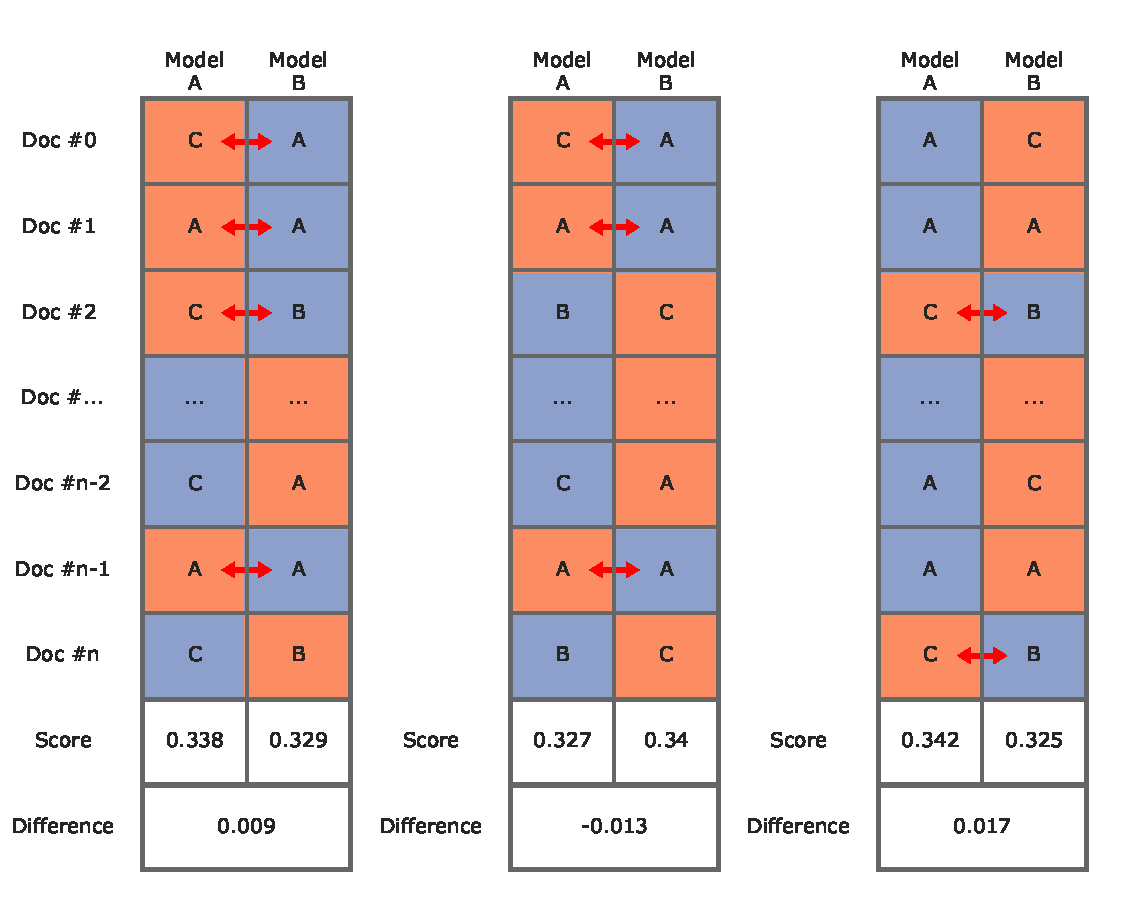
\includegraphics[width=0.51\textwidth]{assets/figures/permutation_test/samples.pdf}\label{fig:permutation_test_samples}}
  \\
  \subfloat[Observed differences in sample scores]{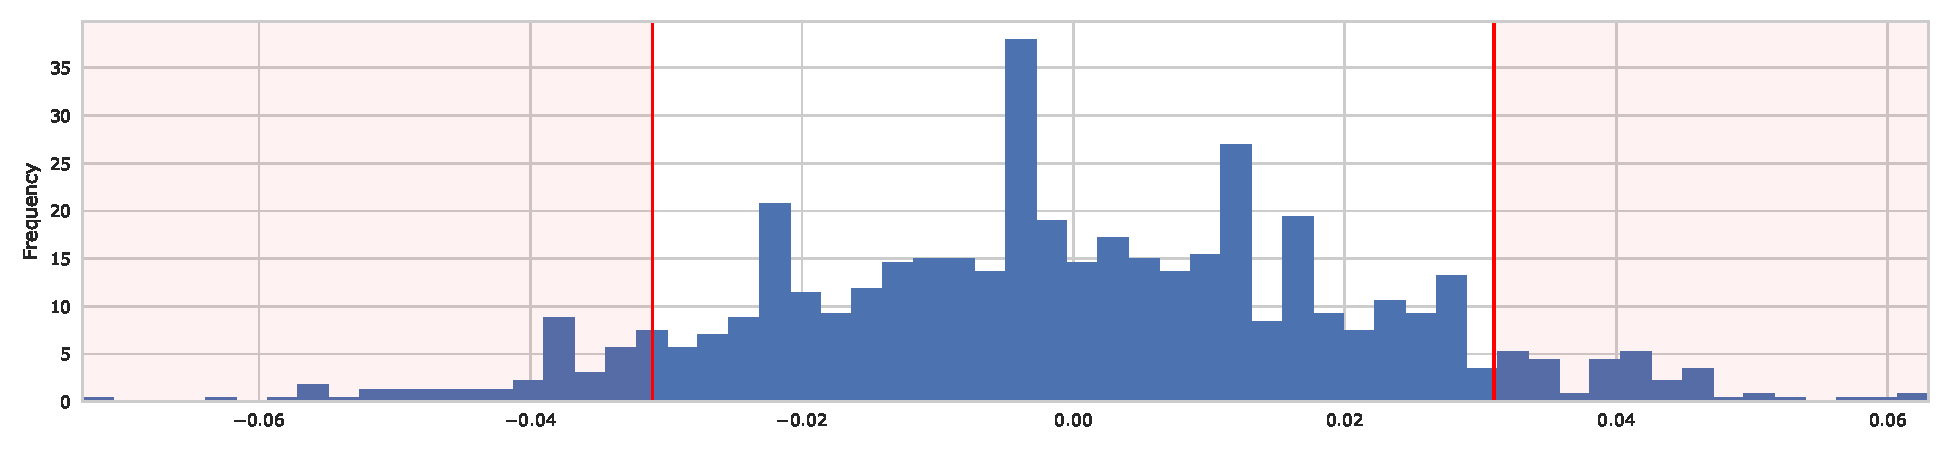
\includegraphics[width=1\textwidth]{assets/figures/permutation_test/distribution.pdf}\label{fig:permutation_test_distribution}}
  \caption{
  Permutation test example.
  A significance test is most often used to test whether a hypothesis is true with a given confidence.
  In this example we use the permutation test to test whether the 
  performance of two given classifiers, Model A and Model B, differs in a non-random way. Our hypothesis is that Model A has a lower performance than Model B, ie. it has a lower score.
  For this example we chose accuracy as the score metric. 
  To calculate the accuracy, we need the true labels, \textbf{\subref{fig:permutation_test_true}}, of the dataset.
  In \textbf{\subref{fig:permutation_test_model_predictions}} we see the predicted labels of the two models and the accuracy as a score beneath them. 
  We also see the difference in the scores.
  In \textbf{\subref{fig:permutation_test_model_predictions}} we also see that Model A has a lower score than Model B.
  This lower score could be due to chance and not because Model B is fundamentally better than Model A.
  To test our hypothesis more throughly we now execute the permutation test.
  In the first step, \textbf{\subref{fig:permutation_test_samples}}, we generate $n$ samples by interchanging the predictions of the two models randomly.
  Here, we depicted three randomly selected samples from the $n$ generated samples.
  To generate a sample, we switch the predictions of Model A and B for every document with a probability of 0.5.
  The switch of two predictions is marked with a red arrow in our depiction.
  In the optimal case, one could generate all possible permutations of the predictions, ie. generate all possible samples.
  Unfortunately this is often not an option due to the sheer number of possibilities. That said, generating a large number of samples also gives a good basis for judgment.
  Next, we calculate the accuracy scores for both models for each of the samples and also calculate the difference between these scores.
  In \textbf{\subref{fig:permutation_test_distribution}} we see the histogram of score differences in the samples.
  The red lines mark the initially observed difference between the models A and B (also it's negative).
  In the last step, we gather these differences and count the number of samples, $n_{higher}$, where the absolute difference between the models is smaller than the score difference of the original predictions of Model A and B.
  $n_{higher}$ divided by the total number of generated samples, $n$, is then the frequency of samples, $f_{higher} = \frac{n_{higher}}{n}$, where the score difference was higher when randomly exchanging the predictions compared to the original observed score difference.
  $f_{higher}$ gives an intuition about the likelihood of observing the difference between the scores of Model A and B.
  In the histogram of observed differences \textbf{\subref{fig:permutation_test_distribution}} this $f_{higher}$ corresponds to the ratio between the area of elements in the blue surface to total area of the histogram.
  In our example, $f_{higher}$ is 0.135, meaning that the probability to observe the score difference we see between the two models is 13.5\% when randomly exchanging the predictions of the two models.
  This is far too high to accept the hypothesis on ground of these predictions.}
\end{figure*}

\todo[inline]{\url{https://stats.stackexchange.com/questions/104040/resampling-simulation-methods-monte-carlo-bootstrapping-jackknifing-cross}}

\labelsubsection{Implementation}{sec:implementation}
For the implementation of all these experiments, we used mostly Python.
\todo[inline]{Scikit-learn, networkx, \dots}
\todo[inline]{Code by Tobias to extract concept maps}

  \refsection{Implementation}{sec:implementation}
  \todo{Scikit-learn, networkx, \dots}
\todo{Code by Tobias to extract concept maps}
  \refsection{Conclusions}{sec:conclusions}
  In our work, we conducted several experiments to test the usefulness of graph-representations of text, especially concept maps, for text classification.
Our experiments ranged from gathering information about the structure of the graphs to actually performing the classification task with different approaches.
For our graph-based classification, we mostly capitalized on graph kernels.
Through all these experiments, we aimed to leverage the particular properties of concept maps, especially the structure.

When directly comparing the performance of graph-based and conventional text-based classification, we saw that the text-only features outperformed the graph-based approach by a high margin, for both co-occurrence graphs and concept maps.
So, our next approach was to combine text- and graph features and classify them together.
This combined approach, while having a far higher runtime due to the increased dimension of the feature vectors, presents no significant improvement of classification scores upon the text-only approach.
On some datasets, the classification score even was a little lower than the text-only approach.
This is also most likely due to the high dimensionality of the combined features and the subsequent risk of overfitting to too specific features.

However, after re-evaluating and extending our graph-based approach, we saw significant improvement in our graph-only classification performance.
Especially splitting the multi-word node labels of the concept maps into single-word nodes resulted in significant improvement on all datasets.
As another extension, we pre-processed the graphs by removing infrequent nodes to further reduce the dimensionality of the resulting feature vectors.
Since we capitalized on the Weisfeiler-Lehman graph kernel to extract our graph features, our guess was that the removal of infrequent words could improve the quality of the features since WL, roughly speaking, counts the matching neighborhoods of nodes.
So, a node label which only occurs infrequently could ``taint" its neighborhood, making an exact match of that neighborhood less likely.
However, when classifying the graphs with the infrequent labels removed, we actually saw mixed results, ranging from great improvements on some datasets to lower scores on others.
Another approach we evaluated was merging infrequent nodes by creating embeddings for each (multi-word) node label using both pre-trained embeddings and creating our own word2vec embeddings from the text.
In the next step, we merged node labels with a similarity above some given threshold.
We then assigned identifiers to the resulting label clusters.
Finally, we relabeled each node in the concept with the identifier of its cluster.
On most datasets, this approach improved the graph-only classification scores.

Besides all these Weisfeiler-Lehman specific extensions and improvements, we also evaluated ``linearizing" the concept maps into text.
By un-rolling the graph into text, we were able to perform text-based classification on them, which - surprisingly - provided the highest classification score we achieved using graphs, for both co-occurrence graphs and concept maps.
For this ``graph kernel" we discarded all structural information since we only used uni-grams, ie. single word frequencies.
In the case of co-occurrence graphs, the performance was nearly as good as the text-only approach, which is not entirely surprising since co-occurrence graphs capture \textit{nearly} all information beside the word order which was not used by our uni-gram \textit{BoW} approach anyway.
For concept maps, the classification scores with this simple linearized graph kernel were also the best, yet still approximately 5-10\% lower in the F1 macro score than both co-occurrence graphs and the text-only approach.

We subsequently repeat the experiments of text- and graph combined features with our extensions, eg. the multi-word label splitting or the relabeling.
Here, interestingly, the classification performance was lower than without these extensions, so with the plain WL graph kernel.
This observation is somewhat surprising since these extensions all improved the classification score when only classifying the graphs.
One possible explanation is, that all these WL extensions aim to transform the concept maps into graphs where the neighborhoods are equalized, ie. more similar to each other.
For instance, the relabeling extension aims to merge infrequent with frequent labels, in order to increase the likelihood of same neighborhoods.
On the other hand, doing this also removes (structural) information from the concept maps, which can not be used for text classification.
For the multi-word label splitting extension, one possible explanation for the lower classification performance when combining the resulting features with text features, is, that it significantly increases the dimensionality of the feature vectors created by WL.
This, in turn, might have lead to overfitting.

Apart the graph kernel customizations we devised for the concept maps, eg. splitting the labels or using directed instead of un-directed edges, we also proposed our own extension to WL, namely node weighting.
Here, our intuition was taken from the fact that WL matches of big neighborhoods are far more difficult than with low-size neighborhoods.
Since this issue is not explicitly encoded in the feature maps of WL, we proposed to scale each feature map entry, corresponding to the label of a node, with a node weight, eg. the degree of that node.
That way, the importance, or frequency, of a node is also encoded in the feature map.
Although this resulted in lower classification scores for our concept map datasets, we saw significant improvement on datasets obtained from \cite{Kersting2016}.
However, a more throughout analysis would be appropriate to confirm the usefulness of our WL extension.

Beyond all the different approaches and experiments, the importance of evaluating the classification scores on different datasets became clear immediately.
One approach leading to a great improvement on some datasets, might actually lead to far lower scores on other datasets.
This once more highlights the importance of appropriate model-selection per dataset, especially when using a graph-based approach.
Understanding the trade-offs of different graph kernels is crucial to achieve higher performance.
The information graph kernels capture varies widely, ranging from simple counts of node labels to more sophisticated structural information.
Therefore, knowing the structure and particularities of the processed graphs is essential to achieve higher classification performance.
In our case, the graph kernel that performed best actually translated the graphs back into text.

Even though we were not able to augment the text-based classification toolbox by another approach, that is graph-based features, we nonetheless explored a number of extensions to existing graph kernels which could be useful for other graph-based tasks.
In our work, we started from text, created graph representations and then classified them to evaluate the usefulness of graph representations in text classification.
However and importantly, concept maps and other graphs can also be created from scratch or extracted automatically from non-text sources, eg. knowledge databases.
While text is currently arguably the most important information medium, maybe - with the rise of more interactive media - concept maps become of greater importance in the future.
There are several advantages of concept maps over text.
For instance, to understand a paragraph at the end of a text, one often must have read the preceding text.
Relations between concepts in a text are often implicit and have to be inferred from the context.
For a reader, a mental picture of the content of the text therefor must carefully be created by the author of the text.
Several levels of detail have to be assessed and introduced by the author, thoughtfully connecting concepts.
In concept maps, on the other hand, concepts have explicit relations to each other.
One can start at every node of a concept map and explore the relationships between concepts by following edges.
This enables the non-linear and visual exploration of the topic of a concept map.
Apart from that, one might also imagine creating concept maps with different levels of details, therefor adding the possibility to add/remove parts of the graph based on their level of detail.
One can think of guided tours through concept maps where parts of the graphs get revealed after each other.
The interactive possibilities of concept maps are numerous, the key being their easy modifiability.
While adding information to texts can be quite laborious since one must find the appropriate section in the text where to add the new parts, with concept maps, on the other hand, extending the graph is as easy as adding a new node or edge to the graph.
Merging multiple concept maps with common concepts is also far easier since one must \textit{only} merge common nodes/concepts.
All these properties and possibilities lead to our opinion that concept maps will become an important information medium alongside text.
Not only side by side, but also a merging of the two mediums is conceivable.
For instance, concept maps could not only have nodes with single labels but assigned texts, images and so on.
Several fields could greatly benefit from concept maps, not only in the learning context \cite{Novak1984}.

\todo{comparison\_combined}
%So, while we were not able to achieve a classification score improvement by augmenting text classification with concept map based features, our observations and approaches nevertheless can be useful for other, graph-related tasks.

\labelsection{Future Work}{subsec:future_work}
There are several aspects which have not been covered in this work.
New graph kernels and approaches to graph processing appear constantly.
These new approaches could also be explored in their usefulness for text-classification.
In our work, we capitalized on the Weisfeiler-Lehman graph kernel, not only because its ability to extract explicit feature maps which in turn could be combined with text features, eg. from BoW.
We proposed an extension to the WL kernel where we augment the plain WL with node weights. Here, it would be interesting to further evaluate the usefulness of this extension on other datasets and with additional normalization.
That said, there are numerous other graph kernels which might prove to be more useful for our task than WL.
Applying them with their different extensions to better suit the particularities of concept maps could result in the performance improvement which we were not able to achieve with our approach.
As we have seen, selecting an appropriate graph kernel is of high importance when doing kernel-based graph processing.

Exploring the differences of concept maps of different datasets could also provide useful insights and improvements for the creation of concept maps.
As we saw, the performance and different graph kernels, and their extensions, resulted in often widely varying classification performance on different datasets, despite fact that the concept maps were all generated by the exact same algorithm.
Finding correlations between the classification performance and properties of concept maps might give new ideas for more suited graph kernels for the classification task.

In our work, we mainly explored concept maps as a text representation.
However, there are a number of other structured representations, not limited to co-occurrence graphs or (semantic) parsing trees.
These other graph representations might also capture structural information about the underlying text and could be interesting candidates for further exploration.
Here, the idea is also to specially leverage the particularities and structures of the graphs.

As a more far-fetching idea, one could also research how the modifiability and composability of concept maps can be harnessed more effectively in the learning context to enable more personalized learning experiences.
For example, when a person wants to learn about some topic using a concept map, he/she most likely has some previous knowledge about that topic.
Providing him/her the same information as everyone else might be the traditional way to go. 
However, providing the person with a more personalized concept map could prove to be useful in removing a lot of information overhead and enhance the learning experience.
Such a personalized concept map could, for example, omit information the user has explored before and has previous knowledge about.
Or, add connections to other topics the person already knows as an entry point.
Also, learning the learning preferences of a user, or giving him options to easily modify/extend a given concept map (semi-) automatically could benefit concept maps becoming a more important information medium.
Observations about the behavior of users of such a learning system in turn could give better insight into possible improvements to automatic concept map creation.
For all this, the key difference to text as an information medium is that concept maps are easily modifiable and composable.
In this idea we envision here, the concept maps could all be interconnected, effectively creating a big knowledge network in which the user can explore given topics in a non-linear way.
Here, a new task arises, namely to classify subgraphs of the big concept map which can provide an entry point for a given topic, maybe also under user-provided constraints, eg. the previous knowledge of the user.
Another task would entail further summarizing concept maps, effectively changing the level of detail.
For example, given three concepts $c_1$, $c_2$, and $c_3$, where $c_1$ is connected to $c_2$ and $c_2$ to $c_3$, how can we remove node $c_2$ and add an edge from $c_1$ to $c_3$ in a meaningful way.
In this example, if the two concept $c_1$ and $c_3$ are important concepts and $c_2$ is less important by some metric, eg. its node degree or some metric of abstractness/detail, this procedure could lower the level of detail of the concept map.
This in turn could enable the interactive exploration of concept maps with varying levels of details.
\todo{Specially try to leverage knowledge bases to connect connected components to each other}
So, instead of approaching the topic of concept maps as yet another way to represent text, this proposed idea would really leverage the particularities and advantages of concept maps and graphs in general.
Utilizing these aspects in learning contexts might then improve the usefulness of concept maps in other domains.

\todo{More detailled error analysis}
\todo{Add stemming/lemmatization to multi-word splitting}

%\todo{Mention \cite{Valerio2007} and their approach (``Reverse" classification: given a document, find a concept map)}




  \newpage
  \printbibliography
\end{document}
